%% Copyright (C) 2020 by
%%   Robert L. Read <read.robert@gmail.com>, Megan Cadena <megancad@gmail.com>,
%%   Juan E. Villacres Perez <jvillacres@utexas.edu>
%% Licensed under Creative Commons Attribution-ShareAlike 4.0 (CC BY-SA 4.0)
%% https://creativecommons.org/licenses/by-sa/4.0/


\documentclass[conference]{article}
\usepackage[backend=biber]{biblatex}
\usepackage{hyperref}
\usepackage{amsmath}
\usepackage{amssymb}
\usepackage{mathtools}
\usepackage{draftwatermark}
\usepackage{outlines}

\addbibresource{work-on-the-airway.bib}

\SetWatermarkText{DRAFT}
\SetWatermarkScale{6}
\SetWatermarkLightness{0.95}

\title{Dynamic-Flow-at-Pressure: A Potentially Useful Concept for Pandemic Ventilators}

\author{Robert L. Read
  \thanks{read.robert@gmail.com}
  email: \href{mailto:read.robert@gmail.com}{read.robert@gmail.com}\\
  Erich B. Schulz
  \thanks{ erich.schulz at mater.org.au}
  email: \href{mailto:erich.schulz at mater.org.au}{erich.schulz at mater.org.au}\\
Megan Cadena
  \thanks{megancad@gmail.com}
  email: \href{mailto:megancad@gmail.com}{megancad@gmail.com}\\
  Juan E Villacres-Perez
  \thanks{jvillacres@utexas.edu}
  email: \href{mailto:jvillacres@utexas.edu}{jvillacres@utexas.edu}
  }


\begin{document}

\maketitle
\begin{abstract}
  Mechanical ventilation must do work on the airway in order to inflate the lungs.
  Considering the power done on the airway may have several uses:
  \begin{itemize}
  \item Computing the maximum required power on the airway in
    a clinical situation provides engineers a minimum power output requirement
    by an air drive mechanism.
  \item Dynamic Flow at Pressure is independent of the means of air production,
    whether by fan, blower, pump, piston, self-inflating bag-squeezer, or bellows.
    It therefore
    may serve as a unifying means of controlling air production to meet
    a clinical goal independent of the means of production.
    \item Developing a predictive model of work enables detection of work done by the patient in either in support (synchronised) or (against) the ventilator.  This may help enable avoidance of problematic patient-ventilator asynchrony and enable fine tuning of ventilation patterns that encourage the patient to work with the ventilator.
  \end{itemize}
  By specifying an {\em air drive} as a modular component in a ventilator
  system that produces air by doing work on the airway according to a
  standardized specification and protocol, it may be possible to
  separate the concern of pressurized medical gas
  prodution from other concerns of building
  ventilators to address the COVID-19 pandemic. This approach improves
  supply chain resilience by allowing air drives to be an interchangable part with
  no need for extensive redesign, testing, and certification.
\end{abstract}


\section{Introduction}

Let us define the term {\em air drive} to mean the mechanism that
produces air and air/oxygen/medical gas mixtures in a mechanical
ventilation system. Because of the
COVID-19 pandemic, many humanitarian engineering teams have
experimented with squeezing inexpensive bag mask valves (BMVs), or
{\em bag squeezers}.
Other mechanisms include pistons, bellows,
positive displacement pumps, which tend to produce a fixed volume against
a variable pressure.
Still other mechanisms such as velocity pumps,
fans and blowers tend to produce a fixed
pressure against a variable back-pressure leading to the injection
of a variable volume. One goal in this paper is to unify these
two very different mechanisms.



\begin{figure}
\begin{center}
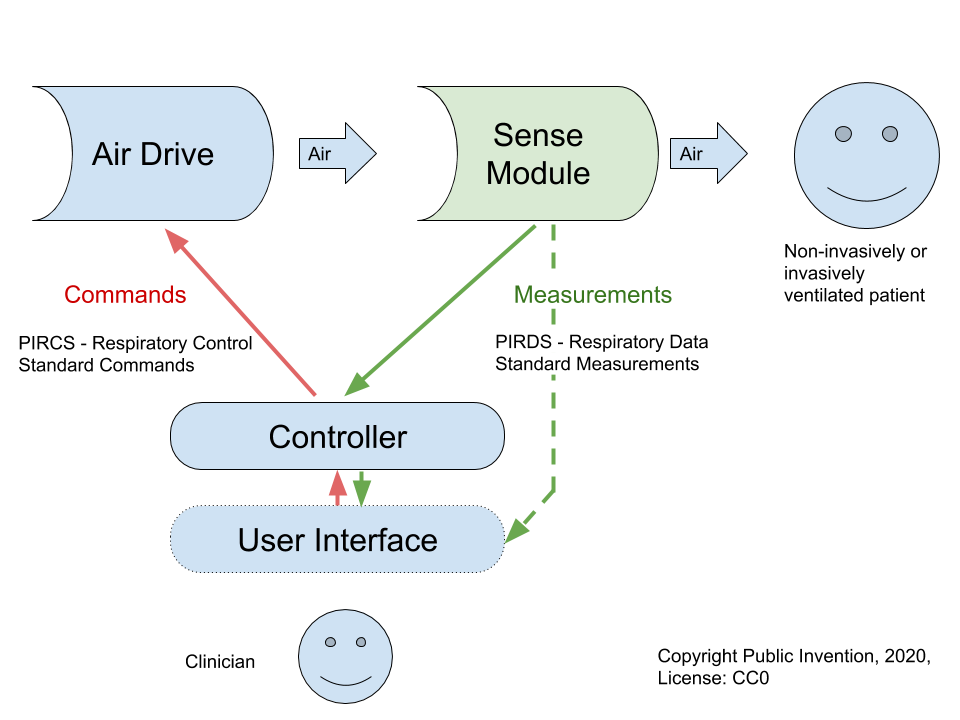
\includegraphics[width=0.9\textwidth]{figures/BasicModules.png}
\caption{A Basic Modular Structure of a Ventilator}
\end{center}
\label{fig:basicmodules}
\end{figure}

A second goal is to champion a modular approach to ventilator design
and construction to better address the COVID-19 pandemic. As of June, 2020,
many teams are independently building new ventilator designs. Cooperation
and division of labor might increase the number of lives saved.
This paper proposes a means of separating the technical problem of precisely
producing medical air on demand from other concerns of building a ventilator.
By providing a standard interface to the ``Air Drive'' module of Figure \ref{fig:basicmodules},
work on that module can proceed independent of other modules.
Finally, creating air drives as a module provides supply-chain resilience.


MIT has presented a useful computation of the work that must be done
on the airway for maximum patient need, from which they conclude a
minimum power requirement for an air drive for
mechanical ventilation\cite{mitpowercalculation}. Expanding on
this work is a second goal of this paper.


\section{Physical Preliminaries}

Roughly speaking, volume times pressure is work.
To inject an infinitesimal amount of air in
to any air vessel or across any air threshold,
the work is the product of the pressure in at the threshold and the
volume injected.
A threshold into a vessel of fixed size is easy to analyze.
A vessel such as a balloon whose volume is dependent on internal pressure
is slightly more complicated.
A rubber balloon has a {\em compliance} which is defined to be
the change in volume with a change in pressure.

A human lung system is even more
complicated, because it has has
both static and dynamic compliance \url{https://en.wikipedia.org/wiki/Lung_compliance}.

Nonetheless, if we use a simplified model, work done over time
on an airway is the integral over time of injected volume
multiplied by pressure, where both injected volume and
pressure are a function of time.

If pressure in the airway is a constant $p$ pascals, a machine which produces a flow of $f$ cubic meters
per second, the machine is perforning $p \cdot f$ watts on the airway.


\section{Ventilation Modes}

Mechanical ventilators offer a number of control modes,
broadly divied into pressure-controlled and bolume-controlled modes.
Modern ventilators typically also provide modes that attempt to support, synchronise with, the patients' own respiratory efforts.
They patient may fight against the action of the ventilator,
called dys-syncrhony. However, if we disregard this clinically
important problem, the modes are simple.

Pressure control mode create inspiration by providing air
at an approximately fixed pressure for a fixed period of time.
In response the flow rate reduces over the course of the inspiratory
phase and lungs fill up and compliance reduces.
Volume control mode pushes air at a constant flow rate for a predetermined length
of time, thus delivering a specified volume with each breath.
As a result the pressure within the system gradually increases to potentially
variable peak pressure unless a preset but limited to some maximum pressure is achieved.


Volume control mode is easy to achieve with a piston which is
powerful enough: use the piston to push the desired volume of
air out of a cylinder and into the airway. (A weak piston might
not be able to do this.) In so doing we may control the speed
of this push which will somewhat control the pressure.
A positive-displacement pump with a small chamber may be pumped
many times to achieve the desired volume; in this say a
piston and positive-displacement pump are similar.

\section{Human Breathing Requirements}

The ranges of pressures, flows, and volumes and the precisions with which
they must be controlled to ventilate a sick human being may surprise
mechanical engineers, and help us contextualize the problem.
Healthcare workers genarlly use cm $H_2O$ as measure of physiological
pressures.

For the designer of pandemic repsonse ventilators, the maximum pressure,
flow and respiration rate the machine should support is of critical importance.
General medical consensus is:
\begin{itemize}
\item Maximum ventilaton volume in one minute is 10 liters (typically 6 liters).
  (Note: A large healthy person exercising heavily may have a normal minute ventilation of 40 liters, but an ill person cannot need that much ventilation.)
\item Maximum pressure needed to for ventilation is 45 cm H2O\cite{de2012large,bein2016standard,australiarequirement}.
  (Note: 80 cm H2O may be used test equipment, but not on a patient.
  The UK HRMA Rapidly Manufactured Ventilator stanadard mentions 35 cm H2O maximum with a 70 cm H2O in exceptional circumstances\cite{rmvs}.)
\item The Australian goverment recommends a maximum instantaneous flow rate of 100 liters per mintues \cite{australiarequirement}.
\item A high-oxygen environment should be assumed. Engineers need to plan for anything
  in contact with medical air to be safe at 50\% or 100\% fractional oxygen (FiO2).
\item A maximum respiratory rate of 30 breaths per minute \cite{rmvs}.
  \item Maximum ratio of Inspiraiton to Expiration (I:E) is 1:1, and generally its is 1:2 or 1:3, with a minimum of 1:5.
  \end{itemize}



\section{Power Calculation}

The inspiring MIT E-Vent Power calculation\cite{mitpowercalculation} performs
a pressure-based evaluation, because the Ambubag is guaranteed to have a volume greater than tidal volume (800ml) they apply.

However, by considering maximum needs, the problem is simplified. In mechanical ventilation,
we can choose a maximum pressure of 50 cm H2O and maximum momentary flow rate of 100 liters per minute.
(This may be a conservative overestimate of the maximum power ever needed in a medical emergency.)
Converting to SI units, we convert the pressure of 45cmH2O to 4413 Pa and 100 lpm to 0.0017 cubic meters per second.
The maximum momentary power on the airway required is the product, 7.355 watts.
(To convert x cmH2O at a flow rate of y lpm, calculate $x \cdot y \cdot 0.00163433333$ watts)
Following the MIT team, we can conclude, for this choice of clinical conditions, any
machine must provide at least 7.35 watts of power instanaously.

Note however, that that is a maximum instaneous power of breathing. Because of the I:E ratio which corresponds to a duty cycle for the machine
and because under normal
conditions the breathing pressure will be much lower than 45 cm H2O, the power of breathing over a full minute
maybe 200 times lower:
\begin{quote}
In a normal person, at rest the work of breathing is about 0.35 J/L, and the power of breathing is about 2.4 J/min (0.04 watts)\cite{mancebo1995comparative}.
\end{quote}

\section{Why use Power-on-the-Airway instead of Flow-at-Pressure?}

Power-on-the-airway ($P$) is the product of flow-into-the-airway ($F$) times
current airway pressure ($A$):
\begin{equation}
  P = F \cdot A
\end{equation}
It is difficult to precisely and safely control ventilation without knowing the
pressure in the airway ($A$) due to the extreme danger of barotrauma.
Therefore one can ask,
``Why not discuss flow-at-pressure instead
of power-on-they-airway?''
Since they are mathematicallly interchangeable, it is
largely a matter of style. Power-on-the-airway has the advantage of being
more relevant to mechanical engineers when operating on certain direct power devices.
Flow-at-pressure makes more sense when considering pressure-release devices.
In order to create a usable standard, we somewhat arbitrarily choose power-on-the-airway
as the most useful to ventilator builders. It is important to note that clinicians
should never need to know about this standard. We hope to insulate the doctor and
patient from this decision, just as at some level they do not know or care what voltage
is used internally by a device.

While it is possible that tracking changing patterns of work may assist doctors to track the progress of the disease, interpretation of trends will be difficult.

The matter is complicated by noise generated by patient muscular efforts and other sources.
Patients may randomly breath in or out in a non-rhythmic (and thus non-predictable manner),
as well randomly cough, sigh, hiccough or even yawn. These patterns will cause breath-to-breath
variation in apparent work done over the course of individual breath cycles.
Alterations in patients level of consciousness and fluctuating levels of experienced pain will cause additional variation.

It is possible that calculating the discrepancy between predicted and actual work performed may provide
some useful clinical insights by quantifying the work done by the patient and the degree of synchronisation
between patient and ventilator. The latter may be useful to assist algorithms better manage patient-ventilator asynchrony.


\section{Practical Air Drive Components}

Air flow may be produced by three basic mechanisms practical for addressing the pandemic.

\begin{outline}
  \1 Pressure producing devices:
  \2 Fans and blowers
  \2 Centrifugal pumps
  \1 Volume producing devices:
  \2 Positive displacement pumps
  \2 BMV squeezers
  \2 Pistons
  \2 Bellows
  \1 Pressure releasing devices:
  \2 Electronically controlled valves,
  \2 Fulidically controlled devices.
\end{outline}


\subsection{Pressure Producing Devices}

Pressure producing devices include fans, blowers, and centrifugal pumps, which
all use a rotary motor to spin blades. The differ in blade configuration and
housing.

In practice, the datasheets of fans show the flow of air they proceeed agianst a given pressure. At some pressure,
this flow drops to zero. In general, fans are provide high flow but develop low pressure. They are generally unsuitable
for respiration, which requires lower flow and higher pressure
compared with most applications.


Note the following language from the RespiraWorks team addresses the problem directly:
\url{https://docs.google.com/document/d/1CE33EcGAdlNdnJA9XW9oGD9veOWSuuBIR2MPmKtkjYQ/edit#}

``Our design centers around a low inertia centrifugal blower, currently sourced from CPAP machines. These brushless fans with lifetime lubricated bearings can spin to high speeds very quickly, allowing a fine degree of time-resolved pressure control. At the same time, they can develop pressures well above 40 cmH2O; even accounting for flow losses, our test model exceeds 100 cmH2O.''

``One of our main assumptions is that access to CPAP blowers will be uninterrupted. We believe both that they are sourced in large quantities (the vendors we’ve contacted in China have more than 5,000 in stock), and that they do not present manufacturing difficulties (fundamentally, it is only three injection molded parts and a brushless DC motor).''

One firm, AirFan, \url{http://www.airfan.fr/mfa0300.html}, makes fans for ventilators using a low-inertial centrifugal pump.

\subsection{Volume Producing Devices}

The world is full of positive-displacement pumps and compressors. Diaphragm pumps are particularly suited because
the airway is contained. Typical compressors fill tanks or tires to at least 35 psi = 2460.74 cm H2O,
about 50 times more than the higest medical breathing pressures of 50 cm H2O. A typical compressor to produce a 250 lpm
flow (10 cubic feet per minute) costs more than \$200 and requires more than 1 horesepower (746 watts).

This typical pressure-too-high and flow-too-low situation may be why
many teams have turned to using BMV squeezers, pumps and bellows,
which can be considered positive-displacement pumps with an exceptionally
large displacement that is pumped only once per breath.
These devices have the apparent advantages of visible simplicity and
supply-chain resilience.

A piston presents the problem of producing a reasonably tight seal
without adding harmful lubricants into the high-oxygen airway.
However, since breathing pressures are low, this may be a surmountable problem.
A bellows with a flexible chamber, usually constrained
to remain within a fixed volume, is another alternative.  Both approaches tend to have simple geometries in which the
change in volume can be easily calculated as a function of the change in the piston of fixed part of the bellows, making
it straightforward to compute flow and therefore power-on-the-airway as a function of the position of the motive element.

On the other hand, a bag-squeezer produces difficult to model dynamic
geometry changes which may be highly dependent on potentially
changing elasticity and deformability of the bag material.
It may not be possible to compute change in volume easily.
The MIT paper suggest that power applied to the bag produces
power on the airway in rough proportion, but the constant of proportionality
may change during the squeezing action.
However, it is easy enough to simply measure the volume as a function of
the position of the squeezing apparatus, and thus to use
an MCU to produce accurate power-on-the-airway when demanded.
It is difficult to see how a bag-squeezer could provide precise control
of any kind without either careful calibration
or adaptive control based on rapid pressure measurements [Giseburt].

\subsection{Pressure Releasing Devices}

\begin{outline}
  \1 Pressure releasing devices:
  \2 Electronically controlled valves,
  \2 Fluidically controlled devices.
\end{outline}

A relatively common approach to ventilation is to assume a source of high-pressure air and control the release of this air
into the airway with a solenoid valve. This has even been done with pure fluidic control which has no moving parts
by directing a flowing airstream into or away from the patient.

In such cases the power-on-the-airway is unrelated to power consumed by operation of the valve, and
depends on the pressure and flow from the pressurized source. However, this is irrelevant to the control system.

\subsection{Summary}

To be supply-chain resilient, we would prefer to use commonly available parts.
In general, fans produce too much flow and not enough pressure, and pumps produce too much pressure and not enough flow.
This may be one of the reason for preponderance of ``bag squeezer'' designs in pandemic ventilator projects.
Some blowers designed specifically for CPAP machines have performance better matched to the breathing task.
These may present supply-chain resilience problems.


\section{Building an Air Drive}

If a blower or centrifugal pump is used as the mechanism of an air drive and the speed of the
blower or pump can be controlled by voltage, and air drive could consist of the blower,
a means of digitally controlling voltage or pulse-width-modulation (PWM), an MCU to receive and interpret commands, and
a map of the voltage  or PWM required to produce a given flow/power at all allowable pressures.
Such an air drive does not need a sensor.
It simply a command in terms of watts, calls a subroutine to look up the voltage in a table
or compute it via interpolation or some formula, and outputs the voltage control.

A positive displacement pump would be different. Generally any such pump produces a stable, known volume displacement with each
stroke or rotation. The air drive would take its command in watts, divide the pressure sent by the controller to obtain
the desired flow and then operate itself at a rate necessary to produce the desired flow.

A pressure gating valve would require that the pressure in the tank be known and the behavior of a valve
be completely understand, but in principle it would also compute a desired flow and operate the valve to achieve that
flow. It might, instead, have its own flow sensor and quickly adjust flow rate to the desired value by its own devices.

The whole point of the air drive is that the effect of all these machines will be unimportant or even unobservable
to doctor and patient. It will not matter to them how the work is done.

\section{Specification of a Power-on-the-airway Air Drive}

Conceptually an air drive is an gas-pushing device which can be be controlled by specifying two values:
\begin{itemize}
 \item Watts of work to be done on the airway, and
 \item The pressure of the airway.
\end{itemize}

In practice, these two values must be transmitted electronically to the air drive.
Typically this would be done with an MCU controller that supports I2C, SPI,
or a serial interface.
The information could be encoded at the byte-level or
in a human-readable format like JSON.
Likewise, a physical standard, such as the ISO 22mm airway connector,
would make it easier
in practice for air drives to be truly interchangeable, but
the definition of such protocols to embody this approach
is beyond the scope of this paper.

We assume that when an air drive receives a command, it is required to
do whatever is necessary to produce the specified
watts on the airway if the airway is at the specified pressure.
It is to continue doing this until it receives the next command.

An air drive may or may not have its own ability to sense the pressure in the airway
for its own purposes. It is acceptable for an air drive to be a rather unintelligent
machine that was simply calibrated at manufacture time to produce the required
flow against the specified pressure to produce the required watts.

\section{How to Test a  Power-on-the-airway Air Drive}

The performance of an air drive can be measured with the following values:
\begin{itemize}
\item{power producible against maximum pressure,}
\item{duty cycle,}
\item{power accuracy is a percentage,}
\item{command repsonse time: maximum time to accept a new command in ms,}
\item{power response time: maximum change in watts/ms per ms,}
\item{mean time to failures in thousands of hours,}
\end{itemize}


For example, a good air drive for mechanical ventilation would be
able to produces 7.35 watts on the airway at any pressure up to 45 cm H2O within
$\pm 0.8 watts$, operate at a
50\% duty cycle, and have a response time 0.2 Watt/ms, reconfigurable every 10ms.
Such a response time
would allow the air drive, operating against a suitable mechanical system such
as a test lung, to generate 45 cm H2O pressure at 100 lpm in 37 ms, and
to release that pressure to zero when so ordered in 37 ms.
It could reliably perform this work for thousands of hours at a duty cycle of 50\%.

The resonse time is clinically important in order to allow efficient ventilation
at high respiration rates.
We do not yet have a mathematical model to understand the impact of low response time,
but clearly if the air drive takes a long time to start doing work on the airway
and a long time to release it, gas exchange and possibly even maximum tidal volume
will be impaired. [See Schulz and Read, Anesthesia.]

To test an air drive, attach the air drive to a pneumatic cylinder. Install a flow
and pressure sensor between the two. Weight or activate the pneumatic cylinder
to produce a range of pressures from 0 to the specified maximum. Command the air drive
to produce a range of powers up to the maximum specified power. Perform this
from a ``standing start'' or zero power and returning to zero power. The response time
can be computed from the pressure and flow curve. At any point in time, power-on-the-airway
is pressure times flows. Measure that the power-on-the-airway is within the specified
accuracy.

If you don't have a pneumatic cylinder, a test lung can accomplish approximately the
same test because it's small volume will quickly be pressurized. This will require
a bit more study of power-on-the-airway to produce pressure, which will be a function
of the restriction on the test lung, compliance, and total volume. Nonetheless it should
be possible by ramping up power to measure all parameters at all pressures.

\subsection{The Importance of Zero Power}

It is important that zero power is a specifiable value which must be met by any
air drive claiming to meet a spec. This situation may be illustrated by a plastic
bag of 1-liter capcity stuffed inside a 500ml glass bottle. Such a model of a lung
would be extreme, but must not be discounted. Such a lung model begins an in
inspiration with extraordinarily
high compliance, which means that a tiny positive pressure makes the first 500ml flow
quickly into the lung model. The compliance then drops to almost zero: not amount of
additional pressure will increase the air in the lung (treating air as imcompressible
and assuming the bottle does not burst.)

However, we take as a principle that within the specifications a doctor should be able
to prescribe any breathing that they see fit for the patient. So, upon reaching 500 ml,
not more positive flow is possible, and therefore no positive work is possible. However,
the air drive must not allow work to be done on it. That is, it must prevent the
back flow of air into the air drive itself, which would be negative power on the airway.
If a doctor says 500ml are to be held statically in the lungs for 1s, the air drive
must be able to accomplish that be so verified, even if it is against zero flow.
This has implications for some mechanical devices which must be considered.

\section{Example Calculations}

\section{Implementing Ventilation Modes With Power-on-the-airway}

In order to accomplish interchangability of air drives within a ventilator without
changing the observable behavior of the ventilator, we imagine a controller which
is sending commands to commands to the air drive.
This controller implements one or more ventilation modes.
The controller represent an algorithm for implementing a ventilation mode
in terms of power-on-the-airway. In almost all cases, the algorithm will use
pressure and possibly flow sensors on the airway that the controller can read.
The air drive may not be able to sense these things itself.

There are a number of ways such an algorithm could be implemented, but
one of the most familiar would be as a PID controller. In the terminology
of such systems, the power-on-the-airway in watts is the {\em control variable},
but the {\em error value} depends on the ventilation mode.

\subsection{Pressure Control Mode}

Pressure Controlled Ventilation (PCV) is perhaps the most basic.
In this mode the error value of the PID controller would be the difference
between the desired PIP and the airway pressure during the inspiration phase,
which is a fixed time, and the difference between the desired PEEP and the
airway pressure during the fixed expiration period. A controller with a single
airway pressure sensor can implement this mode.

\subsection{Volume Control Mode}

Volume Controlled Ventilation (VCV) may assign a fixed flow rate to
performed on the airway until a tidal volume is achieved.
(Generally there remains
a maximum pressure, either implemented mechanically with a pop-off valve,
or electronically.)
Since
flow rate and tidal volume are fixed, the time of inspiration
is calculate by tidal volume divided by flow rate.
Such a mode can be implemented in two ways. If the controller
has a flow sensor, the flow in the airway subtracted from the
prescribed flow can be the error value. However, interestingly, if
we have an airdrive, the controller could implement volume control mode with a single
pressue sensor, by multiplying the desired flow rate times the current pressure
to produce the watts to command the air drive to produce. If the air drive does its
job, the flow will be accurate to with the specified accuracy.

Note that in either case the simple and well-established PID controller
approach can be used.

\subsection{Power-on-the-airway as a clinical measure}

The integration of power over time is work. Although a patient's
lung restriction and compliance may change over time, any inspiration
provided by a power-on-the-airway drive automatically provides
the power of breathing if you simply sum up the watts commanded
and divided by time in each time interval between commands.
A controller using a power-on-the-airway drive thus almost
automaticaly computes the inspiratory work of breathing.

We speculate that it might be clinically valuable to
define a ventilation mode which controls the power-on-the-airway
done in a given insipriation.

\section{Future Work}


\section{References and Notes}

This article: \url{https://pubmed.ncbi.nlm.nih.gov/16857648/}
discusses maximum momentary flow rates for healthy individuals under
heavy exercise, and obtained much higher rates. It also notes that
respirators National Institute for Occupational Safety and Health's respirator test standards of 64, 85, and 100 L/min constant flow
were often exceeded in these circumstances.

Get numbers from here
\url{https://docs.google.com/document/d/1GqadQ2PMJ5qcTDh9ssFBqXj_tbMyajY_QyK9WKKuSOQ/edit#}

What the regulators said in their specifications (todo) - UK Coronavirus (COVID-19): RMVS ventilator specification (talks extensively about limiting fresh gas flow from wall supply but silent on expected flow to be delivered to patient),  Australian TGA specification (requires peak flow rates of 100lpm desirably 150lpm), USA FDA Authorisation, and Association for the Advancement of Medical Instrumentation AAMI Emergency Use Ventilator Design Guidance


%% \bibliographystyle{acm}

%% \bibliography{power-on-the-airway}

\printbibheading

\printbibliography





\end{document}


Bein T, Grasso S, Moerer O, Quintel M, Guerin C, Deja M, Brondani A, Mehta S. The standard of care of patients with ARDS: ventilatory settings and rescue therapies for refractory hypoxemia. Intensive Care Med. 2016 May;42(5):699-711. doi: 10.1007/s00134-016-4325-4. Epub 2016 Apr 4. PMID: 27040102; PMCID: PMC4828494. https://www.ncbi.nlm.nih.gov/pmc/articles/PMC4828494/
de Matos GF, Stanzani F, Passos RH, Fontana MF, Albaladejo R, Caserta RE, Santos DC, Borges JB, Amato MB, Barbas CS. How large is the lung recruitability in early acute respiratory distress syndrome: a prospective case series of patients monitored by computed tomography. Crit Care. 2012 Jan 8;16(1):R4. doi: 10.1186/cc10602. PMID: 22226331; PMCID: PMC3396229. https://pubmed.ncbi.nlm.nih.gov/22226331/


``In a normal person, at rest the work of breathing is about 0.35 J/L, and the power of breathing is about 2.4 J/min.''
\url{https://derangedphysiology.com/main/cicm-primary-exam/required-reading/respiratory-system/Chapter%20041/work-breathing-and-its-components#:~:text=Definitions%20of%20work%20and%20power%20of%20breathing&text=Tada.,is%20about%202.4%20J%2Fmin.}
  ``Normal minute ventilation is between 5 and 8 L per minute (Lpm). Tidal volumes of 500 to 600 mL at 12–14 breaths per minute yield minute ventilations between 6.0 and 8.4 L, for example. Minute ventilation can double with light exercise, and it can exceed 40 Lpm with heavy exercise.''
  \url{https://www.acepnow.com/article/avoid-airway-catastrophes-extremes-minute-ventilation/#:~:text=Normal%20minute%20ventilation%20is%20between,40%20Lpm%20with%20heavy%20exercise.}

    Maximum presumed momentary flow rate: 250 lpm (this is flow rate measured by the Sens

    A very important reference:   \url{http://www.ubccriticalcaremedicine.ca/rotating/material/Lecture_1%20for%20Residents.pdf}
      states:
      ``Lung compliance will change with age, body position, and various pathological
entities. Normal adult lung compliance ranges from 0.1 to 0.4 L/cm H20. Compliance is
measured under static conditions; that is, under conditions of no flow, in order to
eliminate the factors of resistance from the equation.''

``In a spontaneously breathing adult, normal airway resistance is estimated at 2 to 3
cm H2O/L/sec.''
